% Provenance (never printed): see sources/outline_sources.md and sources/book1/BRIEFS.md (g7/05).
\chapter{Finding and Fixing Bugs}\label{ch:g7:finding-and-fixing-bugs}

Leo wrote a \omterm{def:g7:functions:function}{function} for the average of his five marks. They are 12, 10, 11,
9 and 11, all between 9 and 12, and his \omterm{def:g4:programs-and-operating-system:program}{program} prints 13.25. Python gave no
warning: it did exactly what Leo wrote, which is not what he meant. Every
programmer writes \omterm{def:g4:programs-and-operating-system:program}{programs} that go wrong; good programmers have a method for
finding out why.

\begin{recall}
Python stops with an \omterm{def:g6:first-python-program:error}{error message} when it cannot carry out a line
(\cref{ch:g6:first-python-program}). A \omterm{def:g6:variables-and-input:trace-table}{trace table} follows the \omterm{def:g6:variables-and-input:value}{values} of the
\omterm{def:g6:variables-and-input:value}{variables}, one row per step (\cref{ch:g6:variables-and-input}). A \omterm{def:g7:functions:function}{function
call} runs the \omterm{def:g7:functions:function}{function}'s body and comes back with a \omterm{def:g6:variables-and-input:value}{value}
(\cref{ch:g7:functions}); a \omterm{def:g7:lists:list}{list} has indices from 0 to its length minus 1
(\cref{ch:g7:lists}).
\end{recall}

\section{Three kinds of error}

\begin{definition}[Bug]\label{def:g7:finding-and-fixing-bugs:bug}
A \emph{bug}\index{bug} is a mistake in a \omterm{def:g4:programs-and-operating-system:program}{program} that makes it behave
differently from what its author meant.
\end{definition}

\begin{definition}[Syntax error, runtime error, logic error]\label{def:g7:finding-and-fixing-bugs:kinds}
A \emph{syntax error}\index{syntax error} breaks the rules of the language:
Python refuses to start the \omterm{def:g4:programs-and-operating-system:program}{program} at all. A \emph{runtime
error}\index{runtime error} happens while the \omterm{def:g4:programs-and-operating-system:program}{program} runs: it starts, then
stops at a line that cannot be carried out. A \emph{logic error}\index{logic
error} lets the \omterm{def:g4:programs-and-operating-system:program}{program} run to the end, but with a wrong result.
\end{definition}

A colon forgotten at the end of a \code{for} line is a \omterm{def:g7:finding-and-fixing-bugs:kinds}{syntax error}. Python
reads the whole \omterm{def:g3:files-and-folders:file}{file} before running anything, so not even the first line runs:

\Needspace*{9\baselineskip}
\omoutput{code/grade-7/05-finding-and-fixing-bugs/outputs/missing_colon_run.txt}{A
\omterm{def:g7:finding-and-fixing-bugs:kinds}{syntax error}: the mark under the line points at the place where the colon
was expected.}\label{out:g7:finding-and-fixing-bugs:missing-colon}

Dividing by zero is a \omterm{def:g7:finding-and-fixing-bugs:kinds}{runtime error}: the first two lines run, and the third
stops the \omterm{def:g4:programs-and-operating-system:program}{program}.

\Needspace*{6\baselineskip}
\omcode{code/grade-7/05-finding-and-fixing-bugs/listings/zero_division.py}{1}{3}{An
average of nothing.}\label{lst:g7:finding-and-fixing-bugs:zero-division}

\Needspace*{10\baselineskip}
\omoutput{code/grade-7/05-finding-and-fixing-bugs/outputs/zero_division_run.txt}{A
\omterm{def:g7:finding-and-fixing-bugs:kinds}{runtime error}.}\label{out:g7:finding-and-fixing-bugs:zero-division}

Leo's average is a \omterm{def:g7:finding-and-fixing-bugs:kinds}{logic error}, the hardest kind: nothing warns, and the
wrong answer looks like any other number. Only a person who knows what to
expect can see that 13.25 is impossible.

\begin{omfigure}
\begin{tikzpicture}[font=\footnotesize, q/.style={draw=black!60, fill=ocBlue!10, rounded corners, align=center, minimum height=0.8cm}, a/.style={draw=black!60, fill=ocYellow!25, align=center, minimum height=0.8cm}]
  \node[q] (s) at (0,0) {Does the\\ program start?};
  \node[q] (t) at (3.6,0) {Does it run\\ to the end?};
  \node[q] (r) at (7.2,0) {Is the answer\\ right?};
  \node[a] (se) at (0,-1.8) {syntax error};
  \node[a] (re) at (3.6,-1.8) {runtime error};
  \node[a] (le) at (7.2,-1.8) {logic error};
  \node[draw=black!60, fill=ocMint!30, align=center, minimum height=0.8cm] (ok) at (10.4,0) {no bug\\ found};
  \draw[-{Stealth[length=2mm]}, thick] (s) -- node[above] {yes} (t);
  \draw[-{Stealth[length=2mm]}, thick] (t) -- node[above] {yes} (r);
  \draw[-{Stealth[length=2mm]}, thick] (r) -- node[above] {yes} (ok);
  \draw[-{Stealth[length=2mm]}, thick] (s) -- node[left] {no} (se);
  \draw[-{Stealth[length=2mm]}, thick] (t) -- node[left] {no} (re);
  \draw[-{Stealth[length=2mm]}, thick] (r) -- node[left] {no} (le);
\end{tikzpicture}

{\small Three questions tell the three kinds of error apart. ``No \omterm{def:g7:finding-and-fixing-bugs:bug}{bug} found''
is not ``no \omterm{def:g7:finding-and-fixing-bugs:bug}{bug}'': it only means that this run gave the right answer.}
\end{omfigure}

\section{Reading an error report from the bottom}

When a \omterm{def:g7:finding-and-fixing-bugs:kinds}{runtime error} happens inside a \omterm{def:g7:functions:function}{function}, Python reports the whole path
that led there.

\begin{definition}[Traceback]\label{def:g7:finding-and-fixing-bugs:traceback}
A \emph{traceback}\index{traceback} is the error report of a \omterm{def:g7:finding-and-fixing-bugs:kinds}{runtime error}: it
\omterm{def:g7:lists:list}{lists} the calls that were under way when the error happened, from the top of
the \omterm{def:g4:programs-and-operating-system:program}{program} down to the failing line, and ends with the name of the error.
\end{definition}

\omcode{code/grade-7/05-finding-and-fixing-bugs/listings/two_calls.py}{1}{13}{An
error two calls deep.}\label{lst:g7:finding-and-fixing-bugs:two-calls}

\omoutput{code/grade-7/05-finding-and-fixing-bugs/outputs/two_calls_run.txt}{Leo's
line is printed; Mia's call fails.}\label{out:g7:finding-and-fixing-bugs:two-calls}

Read a \omterm{def:g7:finding-and-fixing-bugs:traceback}{traceback} from the bottom. The last line says \emph{what} went wrong: a
division by zero. The lines just above say \emph{where}: line 5, in
\code{average}. Going up, each pair of lines is one step back along the path:
\code{average} was called from line 9, in \code{report}, which was called from
line 13, the main \omterm{def:g4:programs-and-operating-system:program}{program}, with an empty \omterm{def:g7:lists:list}{list}.

\begin{omfigure}
\begin{tikzpicture}[font=\footnotesize, x=1cm, y=1cm]
  \foreach \t/\y/\c in {{line 13, in the main program: report(..., [])}/0/ocBlue!10, {line 9, in report: average(values)}/-0.8/ocBlue!20, {line 5, in average: total / len(values)}/-1.6/ocBlue!30} {
    \node[draw=black!50, fill=\c, anchor=west, minimum width=7.2cm, minimum height=0.6cm, font=\footnotesize\ttfamily] at (0,\y) {\t};
  }
  \node[draw=ocRed, fill=ocRed!10, anchor=west, minimum width=7.2cm, minimum height=0.6cm, font=\footnotesize\ttfamily] at (0,-2.5) {ZeroDivisionError: division by zero};
  \draw[-{Stealth[length=2mm]}, thick, ocRed] (8.6,-2.5) -- (7.4,-2.5);
  \node[anchor=west, align=left, ocRed] at (8.65,-2.5) {1. what: read\\ this first};
  \draw[-{Stealth[length=2mm]}, thick] (8.6,-1.6) -- (7.4,-1.6);
  \node[anchor=west, align=left] at (8.65,-1.6) {2. where it failed};
  \draw[-{Stealth[length=2mm]}, thick] (8.6,-0.4) -- (7.4,-0.4);
  \node[anchor=west, align=left] at (8.65,-0.4) {3. who called it,\\ going up};
\end{tikzpicture}

{\small \cref{out:g7:finding-and-fixing-bugs:two-calls} in short: each box is
one call under way, the deepest one at the bottom.}
\end{omfigure}

\section{Tracing}

A \omterm{def:g6:variables-and-input:trace-table}{trace table} by hand (\cref{ch:g6:variables-and-input}) works for a few
steps. For more, the \omterm{def:g4:programs-and-operating-system:program}{program} can trace itself: extra \code{print} lines show
the \omterm{def:g6:variables-and-input:value}{values} as it runs. Here is Leo's \omterm{def:g7:functions:function}{function}, then the same \omterm{def:g7:functions:function}{function} with
tracing lines:

\Needspace*{11\baselineskip}
\omcode{code/grade-7/05-finding-and-fixing-bugs/listings/average_bug.py}{1}{8}{Leo's
average.}\label{lst:g7:finding-and-fixing-bugs:average-bug}

\Needspace*{5\baselineskip}
\omoutput{code/grade-7/05-finding-and-fixing-bugs/outputs/average_bug.txt}{Higher
than every mark.}\label{out:g7:finding-and-fixing-bugs:average-bug}

\Needspace*{13\baselineskip}
\omcode{code/grade-7/05-finding-and-fixing-bugs/listings/average_trace.py}{1}{10}{The
same \omterm{def:g7:functions:function}{function}, with two tracing lines.}\label{lst:g7:finding-and-fixing-bugs:average-trace}

\Needspace*{11\baselineskip}
\omoutput{code/grade-7/05-finding-and-fixing-bugs/outputs/average_trace.txt}{The
trace: the total is right, the division is
not.}\label{out:g7:finding-and-fixing-bugs:average-trace}

The total, 53, is right, so the walk is not to blame. The trace shows the
mistake at once: Leo divides by 4, the number of marks he had last week, not
by the number of marks in the \omterm{def:g7:lists:list}{list}. \code{len(marks)} always counts them:

\Needspace*{11\baselineskip}
\omcode{code/grade-7/05-finding-and-fixing-bugs/listings/average_fixed.py}{1}{8}{The
average, fixed.}\label{lst:g7:finding-and-fixing-bugs:average-fixed}

\Needspace*{5\baselineskip}
\omoutput{code/grade-7/05-finding-and-fixing-bugs/outputs/average_fixed.txt}{10.6,
between 9 and 12, as it must be.}\label{out:g7:finding-and-fixing-bugs:average-fixed}

Once the \omterm{def:g7:finding-and-fixing-bugs:bug}{bug} is fixed, the tracing lines are removed: they were scaffolding,
not part of the \omterm{def:g4:programs-and-operating-system:program}{program}. Starting them with \code{"  trace:"} makes them easy to
find.

\section{The smallest input that shows the bug}

\begin{definition}[Debugging]\label{def:g7:finding-and-fixing-bugs:debugging}
\emph{Debugging}\index{debugging} is finding the cause of a \omterm{def:g7:finding-and-fixing-bugs:bug}{bug} and fixing it.
\end{definition}

The first step of \omterm{def:g7:finding-and-fixing-bugs:debugging}{debugging} is to make the \omterm{def:g7:finding-and-fixing-bugs:bug}{bug} happen again, on purpose. The
second is to make the \omterm{def:g1:what-is-a-computer:input}{input} as small as possible: a \omterm{def:g7:finding-and-fixing-bugs:bug}{bug} seen on a \omterm{def:g7:lists:list}{list} of a
thousand \omterm{def:g7:lists:list}{items} is hard to follow, the same \omterm{def:g7:finding-and-fixing-bugs:bug}{bug} on a \omterm{def:g7:lists:list}{list} of one \omterm{def:g7:lists:list}{item} is
easy. This \omterm{def:g7:functions:function}{function} should return the first word of a sentence:

\Needspace*{10\baselineskip}
\omcode{code/grade-7/05-finding-and-fixing-bugs/listings/first_word_bug.py}{1}{7}{The
first word, with brackets to show where it starts and
ends.}\label{lst:g7:finding-and-fixing-bugs:first-word-bug}

\Needspace*{8\baselineskip}
\omoutput{code/grade-7/05-finding-and-fixing-bugs/outputs/first_word_bug.txt}{Right
twice, then wrong twice.}\label{out:g7:finding-and-fixing-bugs:first-word-bug}

It fails on \code{"Stop"}, a sentence of one word, and on \code{"a"}, the
smallest such sentence: one letter, and the answer is empty. With no space,
\code{find} returns $-1$, and \code{sentence[:-1]} is everything except the
last \omterm{def:g7:strings:string}{character}. The fix handles the case with no space:

\Needspace*{12\baselineskip}
\omcode{code/grade-7/05-finding-and-fixing-bugs/listings/first_word_fixed.py}{1}{9}{One
more case.}\label{lst:g7:finding-and-fixing-bugs:first-word-fixed}

\Needspace*{8\baselineskip}
\omoutput{code/grade-7/05-finding-and-fixing-bugs/outputs/first_word_fixed.txt}{All
four right.}\label{out:g7:finding-and-fixing-bugs:first-word-fixed}

Many \omterm{def:g7:finding-and-fixing-bugs:bug}{bugs} hide at the edges: an empty \omterm{def:g7:lists:list}{list}, a \omterm{def:g7:lists:list}{list} of one \omterm{def:g7:lists:list}{item}, the first or
the last \omterm{def:g7:lists:list}{index}. A fence of $n$ posts has $n - 1$ gaps between them, and
counting posts when you mean gaps, or the other way round, is so common that
it has a name: an \emph{off-by-one} mistake.

\begin{omfigure}
\begin{tikzpicture}[x=1cm, y=1cm, font=\footnotesize]
  \foreach \i in {0,...,4} {
    \fill[ocInk!70] (1.6*\i-0.08,0) rectangle ++(0.16,1.1);
    \node[ocRed!80!black] at (1.6*\i,-0.3) {post \i};
  }
  \foreach \i in {0,...,3} {
    \draw[thick, black!60] (1.6*\i+0.08,0.8) -- (1.6*\i+1.52,0.8);
    \draw[thick, black!60] (1.6*\i+0.08,0.4) -- (1.6*\i+1.52,0.4);
    \node[ocBlue!80!black] at (1.6*\i+0.8,1.3) {gap \i};
  }
\end{tikzpicture}

{\small Five posts, four gaps. A \omterm{def:g7:lists:list}{list} of $n$ \omterm{def:g7:lists:list}{items} has $n - 1$ pairs of
neighbours, and its last \omterm{def:g7:lists:list}{index} is $n - 1$.}
\end{omfigure}

\section{Changing one thing at a time}

\begin{method}[Debugging, one step at a time]\label{met:g7:finding-and-fixing-bugs:cycle}
\begin{enumerate}
  \item \textbf{Reproduce}: find an \omterm{def:g1:what-is-a-computer:input}{input} that shows the \omterm{def:g7:finding-and-fixing-bugs:bug}{bug} every time.
  \item \textbf{Shrink}: make that \omterm{def:g1:what-is-a-computer:input}{input} as small as you can.
  \item \textbf{Guess}: read the error report or a trace, and guess the
    cause.
  \item \textbf{Change one thing}, and run again on the same \omterm{def:g1:what-is-a-computer:input}{input}.
  \item If the \omterm{def:g7:finding-and-fixing-bugs:bug}{bug} is gone, keep the change and run the other \omterm{def:g1:what-is-a-computer:input}{inputs} too;
    if not, undo the change and go back to step 3.
\end{enumerate}
\end{method}

Changing two things at once seems faster, but if the \omterm{def:g4:programs-and-operating-system:program}{program} then works, or
fails differently, you cannot tell which change did it.

\begin{omfigure}
\begin{tikzpicture}[font=\footnotesize, box/.style={draw=black!60, rounded corners, fill=ocBlue!10, minimum width=2.3cm, minimum height=0.7cm}]
  \node[box] (a) at (0,0) {reproduce};
  \node[box] (b) at (3,0) {shrink};
  \node[box] (c) at (6,0) {guess};
  \node[box] (d) at (9,0) {change one thing};
  \node[box, fill=ocMint!30] (e) at (9,-1.6) {run again};
  \draw[-{Stealth[length=2mm]}, thick] (a) -- (b);
  \draw[-{Stealth[length=2mm]}, thick] (b) -- (c);
  \draw[-{Stealth[length=2mm]}, thick] (c) -- (d);
  \draw[-{Stealth[length=2mm]}, thick] (d) -- (e);
  \draw[-{Stealth[length=2mm]}, thick] (e) -| (c);
  \node[anchor=east, align=right] at (5.9,-1.1) {still wrong:\\ undo, guess again};
\end{tikzpicture}

{\small The \omterm{def:g7:finding-and-fixing-bugs:debugging}{debugging} cycle of \cref{met:g7:finding-and-fixing-bugs:cycle}.}
\end{omfigure}

\begin{history}[A real bug]
% ledger: g7:bug-1947
Engineers already called a fault a ``\omterm{def:g7:finding-and-fixing-bugs:bug}{bug}'' long before \omterm{def:g1:what-is-a-computer:computer}{computers}. On 9
September 1947, at Harvard, in Cambridge, Massachusetts, the operators of
the Mark II, a \omterm{def:g1:what-is-a-computer:computer}{computer} built from electrical switches called relays, found a
moth caught in one of them. They taped it into the machine's log book with
the words ``First actual case of \omterm{def:g7:finding-and-fixing-bugs:bug}{bug} being found''.
\end{history}

\begin{omfigure}
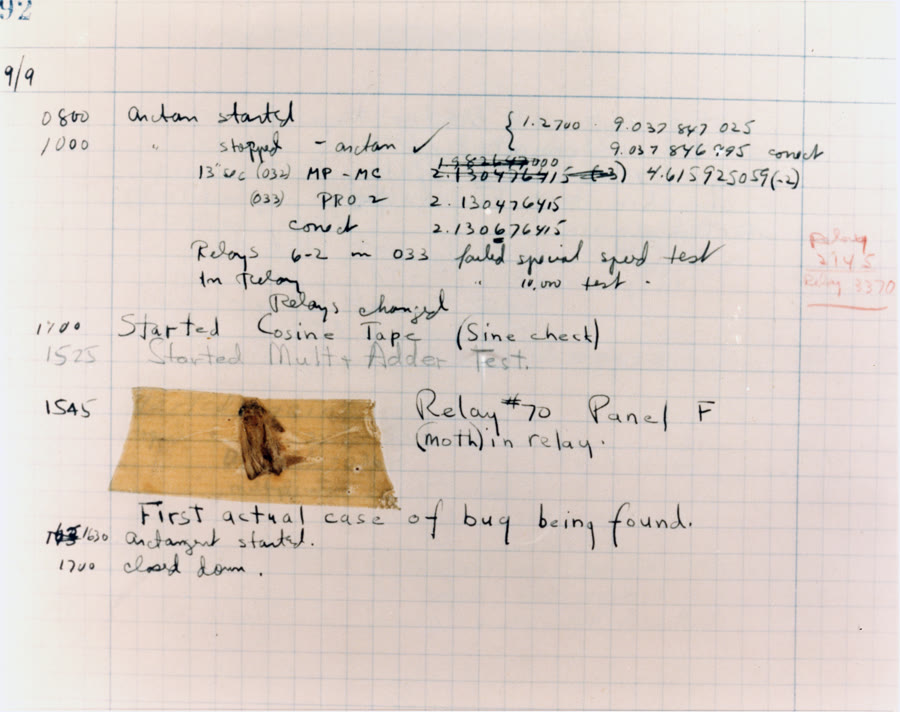
\includegraphics[width=0.6\linewidth]{images/book1/g7-first-bug.jpg}

{\small The log-book page of 9 September 1947, with the moth taped under the
time 15:45.}
\end{omfigure}

\section{Exercises}

\begin{exercise}[$\star$]\label{exo:g7:finding-and-fixing-bugs:1}
Which kind of error is each of these: (a) a missing bracket; (b) a \omterm{def:g7:lists:list}{list} \omterm{def:g7:lists:list}{index}
past the end; (c) a price total that is 10 times too big; (d) a word spelt
\code{pritn}, on a line that runs; (e) a \omterm{def:g4:algorithms-repeat-and-decide:loop}{loop} that counts one \omterm{def:g7:lists:list}{item} too
few; (f) a \code{while} \omterm{def:g4:algorithms-repeat-and-decide:loop}{loop} with \code{whle}?
\end{exercise}

\begin{exercise}[$\star$]\label{exo:g7:finding-and-fixing-bugs:2}
Here is a \omterm{def:g7:finding-and-fixing-bugs:traceback}{traceback}. What went wrong, on which line, and inside which
\omterm{def:g7:functions:function}{function}?

\omoutput{code/grade-7/05-finding-and-fixing-bugs/outputs/last_item_run.txt}{An
error report to read.}\label{out:g7:finding-and-fixing-bugs:last-item}
\end{exercise}

\begin{exercise}[$\star$]\label{exo:g7:finding-and-fixing-bugs:3}
In \cref{out:g7:finding-and-fixing-bugs:average-trace}, which lines come from
the tracing lines? What remains once they are removed?
\end{exercise}

\begin{exercise}[$\star$]\label{exo:g7:finding-and-fixing-bugs:4}
Tom's \omterm{def:g4:programs-and-operating-system:program}{program} stops with \code{SyntaxError: '(' was never closed} on the
line \code{print("count:", len(marks)}. Fix it.
\end{exercise}

\begin{exercise}[$\star\star$]\label{exo:g7:finding-and-fixing-bugs:5}
This \omterm{def:g4:programs-and-operating-system:program}{program} should add the first five marks, but prints 67. Why? Fix it.

\omcode{code/grade-7/05-finding-and-fixing-bugs/exercises/first_five.py}{1}{5}{One
mark too many.}\label{lst:g7:finding-and-fixing-bugs:first-five}
\end{exercise}

\begin{exercise}[$\star\star$]\label{exo:g7:finding-and-fixing-bugs:6}
This \omterm{def:g7:functions:function}{function} should count the \omterm{def:g6:variables-and-input:value}{values} above \code{limit}; it has a tracing
line. It answers 0 for \code{[3, 9, 7]} and 5. Read the trace and find the
\omterm{def:g7:finding-and-fixing-bugs:bug}{bug}.

\omcode{code/grade-7/05-finding-and-fixing-bugs/listings/count_above_trace.py}{1}{10}{A
count with a trace.}\label{lst:g7:finding-and-fixing-bugs:count-above}

\omoutput{code/grade-7/05-finding-and-fixing-bugs/outputs/count_above_trace.txt}{Only
one line of trace.}\label{out:g7:finding-and-fixing-bugs:count-above}
\end{exercise}

\begin{exercise}[$\star\star$]\label{exo:g7:finding-and-fixing-bugs:7}
Add a tracing line to \cref{lst:g7:finding-and-fixing-bugs:first-word-bug}
that prints \code{end} for each sentence. What does it print for \code{"Stop"}?
\end{exercise}

\begin{exercise}[$\star\star$]\label{exo:g7:finding-and-fixing-bugs:8}
Noor writes \code{if mark =< 10:}. Which kind of error is it, and how is it
written in Python?
\end{exercise}

\begin{exercise}[$\star\star$]\label{exo:g7:finding-and-fixing-bugs:9}
This \omterm{def:g7:functions:function}{function} should say whether a \omterm{def:g7:lists:list}{list} is in order from small to large,
equal neighbours allowed. Find the smallest \omterm{def:g7:lists:list}{list} on which it is wrong, then
fix it.

\omcode{code/grade-7/05-finding-and-fixing-bugs/exercises/is_sorted_bug.py}{1}{9}{In
order?}\label{lst:g7:finding-and-fixing-bugs:is-sorted}
\end{exercise}

\begin{exercise}[$\star\star\star$]\label{exo:g7:finding-and-fixing-bugs:10}
Change the \omterm{def:g7:functions:function}{function} \code{average} of \cref{lst:g7:finding-and-fixing-bugs:two-calls}
so that it returns 0 for an empty \omterm{def:g7:lists:list}{list} instead of stopping the \omterm{def:g4:programs-and-operating-system:program}{program}.
\end{exercise}

\begin{exercise}[$\star\star\star$]\label{exo:g7:finding-and-fixing-bugs:11}
This \omterm{def:g4:programs-and-operating-system:program}{program} should add the even numbers from 1 to 10, which makes 30. It
prints 25 and has two \omterm{def:g7:finding-and-fixing-bugs:bug}{bugs}. Fix them one at a time, running after each fix,
in both orders. Is the final \omterm{def:g4:programs-and-operating-system:program}{program} the same? Then why fix one at a time?

\omcode{code/grade-7/05-finding-and-fixing-bugs/exercises/evens_bug.py}{1}{6}{Two
\omterm{def:g7:finding-and-fixing-bugs:bug}{bugs}.}\label{lst:g7:finding-and-fixing-bugs:evens}
\end{exercise}

\begin{exercise}[$\star\star\star$]\label{exo:g7:finding-and-fixing-bugs:12}
This \omterm{def:g7:functions:function}{function} is right on most \omterm{def:g7:lists:list}{lists} of marks. Find a \omterm{def:g7:lists:list}{list} on which it is
wrong, the smallest one, and fix it.

\omcode{code/grade-7/05-finding-and-fixing-bugs/exercises/largest_bug.py}{1}{6}{The
largest mark?}\label{lst:g7:finding-and-fixing-bugs:largest}
\end{exercise}

\section{Problem: The Bug Hunt}

\begin{problem}[{Weekend problem --- four bugs in a grader}]\label{pb:g7:finding-and-fixing-bugs:1}
A teacher's \omterm{def:g4:programs-and-operating-system:program}{program} gives a quiz score from 0 to 99 a letter (A from 90, B
from 75, C from 50, D below) and a \omterm{def:g6:first-python-program:comment}{comment} from its tens digit (poor below 50,
fair in the 50s and 60s, good in the 70s and 80s, great from 90). It has four
\omterm{def:g7:finding-and-fixing-bugs:bug}{bugs}: one \omterm{def:g7:finding-and-fixing-bugs:kinds}{syntax error}, one \omterm{def:g7:finding-and-fixing-bugs:kinds}{runtime error} and two \omterm{def:g7:finding-and-fixing-bugs:kinds}{logic errors}.

\omcode{code/grade-7/05-finding-and-fixing-bugs/listings/grader.txt}{1}{28}{The
grader, as the teacher wrote it.}\label{lst:g7:finding-and-fixing-bugs:grader}

\medskip\noindent\textbf{Part I --- The errors that stop the program.}
\begin{enumerate}
  \item Before running it, find the \omterm{def:g7:finding-and-fixing-bugs:kinds}{syntax error} by reading.
  \item Here is the \omterm{def:g4:programs-and-operating-system:program}{program} run as it is, then run again with the colon added
    (the \omterm{def:g3:files-and-folders:file}{file} \code{grader_v1.py}). Which line does each report point to?

\omoutput{code/grade-7/05-finding-and-fixing-bugs/outputs/grader_run.txt}{Two
runs, two reports.}\label{out:g7:finding-and-fixing-bugs:grader-run}

  \item Read the second report from the bottom. Which \omterm{def:g7:functions:function}{function} failed, and
    with which score? Which \omterm{def:g6:variables-and-input:value}{value} did \code{tens} have? Fix the \omterm{def:g7:finding-and-fixing-bugs:kinds}{runtime error}.
\end{enumerate}

\medskip\noindent\textbf{Part II --- Checking a hundred scores.} The \omterm{def:g3:files-and-folders:file}{files}
\code{grader_v2.py}, \code{grader_v3.py} and \code{grader_v4.py} are the
grader after one, two and three more fixes. A checking \omterm{def:g4:programs-and-operating-system:program}{program} works out the
expected grade another way and counts the wrong answers:

\omcode{code/grade-7/05-finding-and-fixing-bugs/listings/check_grader.py}{1}{26}{Every
score from 0 to 99.}\label{lst:g7:finding-and-fixing-bugs:check}

\begin{enumerate}[resume]
  \item Why is it safer to check against a second, simpler way of working out
    the grade than against answers typed by hand?
  \item Run it. How many wrong answers does each version give?
  \item Which \omterm{def:g7:finding-and-fixing-bugs:kinds}{logic error} was fixed between \code{v2} and \code{v3}, and
    which one between \code{v3} and \code{v4}?
  \item In Part I, the scores 45 and 75 got the \omterm{def:g6:first-python-program:comment}{comment} ``fair''. Was that
    a sign of a \omterm{def:g7:finding-and-fixing-bugs:bug}{bug}?
\end{enumerate}

\medskip\noindent\textbf{Part III --- The smallest inputs.}
\begin{enumerate}[resume]
  \item Which is the smallest score that shows the \omterm{def:g6:first-python-program:comment}{comment} \omterm{def:g7:finding-and-fixing-bugs:bug}{bug}? Why that
    one?
  \item Which scores show the letter \omterm{def:g7:finding-and-fixing-bugs:bug}{bug}? Which line of the \omterm{def:g1:what-is-a-computer:input}{output} of Part I
    already showed it?
  \item Had the letter \omterm{def:g7:finding-and-fixing-bugs:bug}{bug} been fixed first, how many wrong answers would
    remain? Why not 65?
  \item State the result.
\end{enumerate}
\end{problem}
